\documentclass[a4apaper,twocolumn,10pt]{article}
\usepackage[spanish]{babel}
\usepackage[utf8]{inputenc}
\usepackage{graphicx}
\usepackage{flushend}
\usepackage{textcomp}
\usepackage{amssymb, amsmath, amsbsy} 
\usepackage{hyperref}
\usepackage{graphicx}
\graphicspath{ {./Proyecto_final/} }
\usepackage{afterpage}
\usepackage{upgreek}

\begin{document}
\title{Interacción de las erupciones
volcánicas con la atmósfera:
interacciones específicas y el caso hist\'orico del Pinatubo en 1991, con simulaciones clim\'aticas de los a\~nos sucesivos.}
\author{Evelina Dallara}
\date{}
\twocolumn[
\begin{@twocolumnfalse}
\maketitle
\begin{abstract}
Repositorio: \href{url}{https://github.com/Eve16/Proyecto\_final.git}
\\Palabras clave: Erupciones volc\'anicas, atm\'osfera, capa de aerosoles de Junge
\end{abstract}
\end{@twocolumnfalse}
]

\section{Introducción}
Las erupciones volc\'anicas tienen un efecto importante tanto a escala local como global,
considerando la superficie terrestre como la atm\'osfera. Los efectos sobre esta \'ultima pueden causar cambios importantes en el clima, a peque\~nos y grandes intervalos de tiempo, afectando de manera diferente a la sociedad. Las interacciones entre la columna eruptiva y la atm\'osfera se pueden observar de distintas formas, en este caso vamos a considerar principalmente la capa de aerosoles de Junge y la formaci\'on de las nubes cirrus. Además, se va a presentar un caso de erupci\'on hist\'orica que ha tenido un impacto importante a escala global: la erupci\'on del Pinatubo en 1991. Finalmente se presentar\'an los resultados de la modelizaci\'on climatica de los dos a\~nos despu\'es de la erupci\'on. 
\section{Efectos sobre la capa de aerosoles de Junge}
La capa de aerosol de Junge es un estrato global situado a unos 20 km de altitud que refleja la luz solar y por tanto lleva a un enfriamiento de la atm\'osfera inferior, as\'i como a un calentamiento local por la absorci\'on de la radiaci\'on \cite{von2009effects}. Se ha podido observar como las erupciones explosivas que llegan a alcanzar esta altitud tienen un importante impacto sobre esta \'ultima capa, debido mayormente a la emisi\'on de sulfuros. Estos sulfuros, emitidos en forma de $SO_{2}$ se oxidan formando el $H_{2}SO_{4}$, que puede llevar a un aumento de los aerosoles de sulfato l\'iquido y que pueden permanecer en la atmósfera durante años
\cite{vernier2011major}. La oxidaci\'on de este \'ultimo se produce seg\'un las ecuaciones 
\begin{displaymath}
OH+SO_{2}\rightarrow HSO_{3}
\end{displaymath}
\begin{displaymath}
HSO_{3}+O_{2}\rightarrow SO_{3}+HO_{2}
\end{displaymath}
\begin{displaymath}
SO_{2}+2H_{2}O\rightarrow H_{2}SO_{4}+H_{2}O
\end{displaymath}
Uno de los ejemplos más significativos del efecto de una erupción volcánica sobre la
capa de Junge ha sido la erupción del Pinatubo en 1991. Durante esta erupci\'on los 20 Tg de $SO_{2}$ que habían sido emitidos llegaron a la capa de Junge y causaron un enfriamiento de la
temperatura global de unos 0.4 \textdegree C en el a\~no después de la erupción y un calentamiento de la estratosfera inferior de 1.5 \textdegree C. Además, después de esta erupción, los aerosoles volcánicos han sido transportados hacia latitudes mayores donde se produjeron reacciones que llevan a la formación del agujero del ozono. Con el tiempo los aerosoles disminuyen debido a
sedimentación e intercambios entre la estratosfera y troposfera, así que la estratosfera llega de
nuevo a estar en condición no-volcánica. De hecho, en ausencia de erupciones volcánicas la
presencia de la capa de Junge se relaciona con la emisión en la superficie de precursores de
gases sulfúricos

\section{Consecuencias en la formación de los cirrus}
Los cirrus son nubes que se forman en la capa superior de la troposfera, el estrato de la
atm\'osfera que va desde la superficie terrestre hasta unos 10 km de altitud, a trav\'es de cristales de hielo que crecen sobre n\'ucleos que suelen ser part\'iculas de arena o met\'alicas. Adem\'as, estas nubes tienen un efecto mayor sobre las radiaciones con longitudes de ondas grandes, causando
as\'i un mayor calentamiento de la superficie terrestre. Resulta importante conocer si los
aerosoles en la estratosfera provenientes de erupciones volc\'anicas tienen alg\'un efecto sobre la formaci\'on de los cirrus. \cite{friberg2015influence} ha estudiado esta relaci\'on y observ\'o una variaci\'on de las concentraciones de sulfuros en la parte inferior de la estratosfera (LMS) y capa
superior de la troposfera (UT) dependiendo de la estaci\'on del a\~no. Es importante tener en cuenta tambi\'en que la concentraci\'on de sulfuros aumenta desde los tr\'opicos hacia latitudes mayores. Mientras que, si consideramos latitudes medias vemos como en la LMS hay altos valores de S/PV, que es la raz\'on entre sulfuros y potencial de vorticidad, durante la primavera que despu\'es disminuye en verano, con un m\'inimo durante agosto-octubre. 
\begin{figure}[t]
\centering
  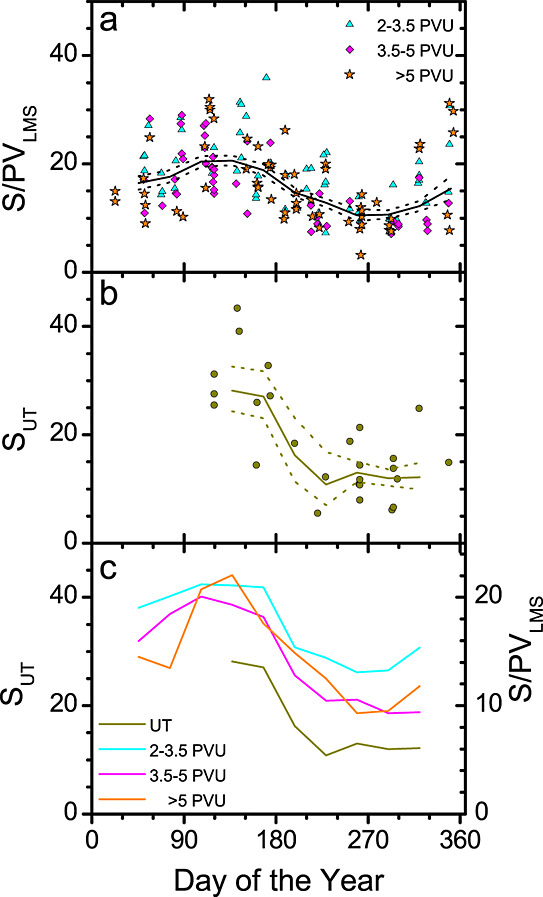
\includegraphics[width=0.25\textwidth,height=6cm]{Figura1}
  \caption{Cambios estacionales en (a) S/PV en diferentes intervalos de PV en la LMS, (b) las concentraciones de sulfuros en la UT, y (c) comparación directa del S/PV en la LMS y sulfuros en la UT.}
  \label{fig:Figura1}
\end{figure}
El m\'aximo coincide con el flujo de aire descendiente desde la estratosfera hacia la LMS, done se forman los cirrus,
que lleva consigo las part\'iculas de sulfuros, este movimiento de aire se denomina circulaci\'on de Brewer-Dobson (BD). En la Figura \ref{fig:Figura1} se puede observar la existencia de una similitud entre las variaciones de concentraciones de sulfuros en los casos de la LMS y de la UT, lo que indica una fuerte relacin\'o entre las dos concentraciones en aerosoles que puede estar influenciada por la actividad volc\'anica. Por tanto, se puede decir que la variabilidad de los sulfuros est\'a causada por la variaci\'on estacional debido al movimiento de las masas de aire y por las contribuciones de aerosoles volc\'anicos. En general, un aumento de los aerosoles lleva a un incremento de las part\'iculas que pueden fingir como n\'ucleos para la condensaci\'on, disminuyendo el tama\~no y entonces aumentando de consecuencia la capacidad de reflejar la radiaci\'on (aumento del albedo de la nube).

\section{Caso erupción Pinatubo 1991}
El 15 de junio de 1991 se produjo la erupci\'on del Mt Pinatubo, con la consecuente
producci\'on de una columna eruptiva que alcanz\'o los 30 km de altitud. Esta \'ultima aport\'o una gran cantidad de $SO_{2}$, que al reaccionar con la estratosfera se transform\'o en $H_{2}SO_{4}/H_{2}O$, con una
masa resultante de aerosoles de unos 30 Tg, considerado como la mayor perturbaci\'on de la estratosfera del \'ultimo siglo \cite{mccormick1995atmospheric}. La nube de esta erupci\'on ha sido ampliamente estudiada con numerosos m\'etodos y ha sido observada su importante influencia sobre las concentraciones de $NO_{2}$, cloro reactivo y ozono. Estaba constituida por vapor aqueo,
gases sulf\'ureos y aerosoles, concentr\'andose en una altitud entre los 20 y 27 km logr\'o dar la vuelta al mundo en 22 d\'ias. En la Figura \ref{fig:Figura2} vemos la evoluci\'on de los aerosoles producidos por este evento eruptivo, obtenido a trav\'es del instrumento de ocultamiento solar SAGE II.
\begin{figure}[t]
\begin{center}
  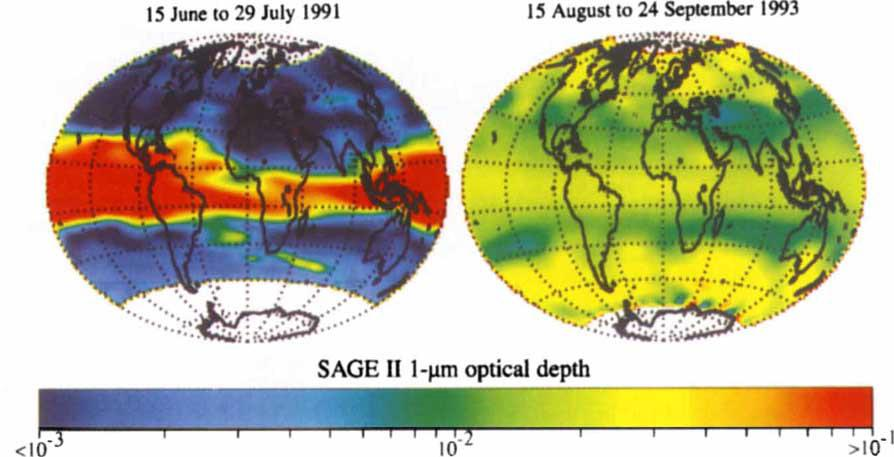
\includegraphics[width=0.5\textwidth,height=6cm]{Figura2}
  \end{center}
  \caption{Desarrollo y dispersi\'on de los aerosoles inyectados en la atm\'osfera durante la erupci\'on del Pinatubo y monitorizados por distintos sat\'elites.}
  \label{fig:Figura2}
\end{figure}
El movimiento de la masa de aerosoles en este caso se desplaz\'o desde los tr\'opicos de
manera muy lenta, un hecho que parece ser una caracter\'istica muy com\'un de las grandes
erupciones a bajas latitudes. De hecho, el transporte de los aerosoles hacia los polos se produce m\'as dif\'icilmente con la presencia de vientos del este en zonas ecuatoriales. En este caso hubo unos vientos del este que dominaban sobre los 23 km durante los primeros seis meses despu\'es
de la erupci\'on. Sin embargo, a altitudes menores los aerosoles se desplazaron m\'as r\'apidamente hacia los polos. La disminuci\'on de la concentraci\'on de aerosoles est\'a debido al hecho de que con el tiempo estos son transportados desde la estratosfera a la troposfera donde sufren varios mecanismos que causan su sedimentaci\'on sobre la superficie de la Tierra. De hecho, se observa como a partir del a\~no 1993 la concentraci\'on disminuye. Debido a la gran inyecci\'on de sulfuros en la estratosfera se han registrado valores de albedo muy altos durante los meses de julio, agosto y septiembre del mismo a\~no de la erupci\'on.
El aumento de albedo hab\'ia sido detectado tambi\'en en regiones con valores generalmente altos de este mismo, debido a la inclusi\'on de aerosoles en la troposfera superior que, por tanto, interaccionan con nubes convectivas, alterando sus propiedades microf\'isicas. Como hemos visto
anteriormente, el aumento de los aerosoles causa un aumento en el albedo, lo que deber\'ia causar un enfriamiento. Sin embargo, dependiendo de las propiedades microf\'isicas de los aerosoles, se puede producir una absorción en el IR, llevando a un calentamiento por efecto invernadero, o una dispersi\'on de la radiaci\'on solar, produciendo un enfriamiento. Adem\'as, si el
radio de los aerosoles supera los 2$\mu$m el efecto de calentamiento domina y en el caso de la erupci\'on del Pinatubo hubo un incremento de este par\'ametro desde 0.3 a 1 $\mu$m, por tanto, deber\'ia producirse un enfriamiento. Sin embargo, en un primer momento se registr\'o un aumento de la temperatura en la estratosfera, hasta 1992, y hacia el final de 1193 se observ\'o
un enfriamiento en la estratosfera, que se relacion\'o con la p\'erdida de ozono, un absorbedor eficiente de radiaci\'on solar y responsable del calentamiento en la estratosfera.

\section{Simulaci\'on del modelo clim\'atic de los dos a\~nos despu\'es de la erupci\'on}

\afterpage{\null\newpage}
\newpage
\bibliographystyle{apalike}
\bibliography{Bibliografia_6.bib}
\end{document}